\large
A filtered-$x$ least mean square (FXLMS) algorithm is used along with the error microphone, to find the counter phase signal of the  noise.
%The filter coefficients are adapted using the error, measured with microphone (3).
\resizebox{1\columnwidth}{!}{
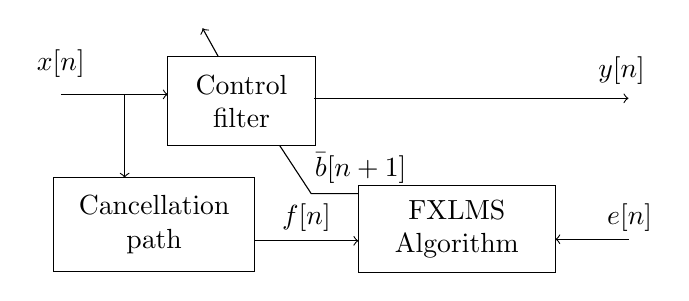
\begin{tikzpicture}
\draw  (-2.9,0.98) rectangle node[text width=2.5cm,align=center] {\textrm{Cancellation \\ path}}(-0.35,-0.21);
\draw  (0.97,0.88) rectangle node[text width=2.5cm,align=center] {\textrm{FXLMS Algorithm}} (3.47,-0.22);
\draw  (-1.45,2.52) rectangle node[text width=1.5cm,align=center,fill=white] {\textrm{Control filter}} (0.42,1.39);
\draw[->] (-0.35,0.18) -- node[above]{$f[n]$} (0.97,0.18);
\draw [->](-2,2.03) -- (-2,0.98);
\draw [->](-2.81,2.04) node[left,above=2.5]{$x[n]$} -- (-1.45,2.04);
\draw[->] (0.41,1.99) -- (1.25,1.99) -- (4.4,1.99) node[left=2.5,above=1.5]{$y[n]$};
\draw (0.97,0.78) -- (0.37,0.78) --node[above=0.55,right=3.5]{$\bar{b}[n+1]$} (-0.03,1.39);
\draw [->](-0.81,2.52) -- (-1.01,2.88);
\draw[->] (4.4,0.2) -- node[above=8,right=2]{$e[n]$} (3.47,0.2);
\end{tikzpicture}
}

%\vspace{-2mm}
%\begin{equation*}
%	b_j[n+1] = b_j[n] - 2\mu e[n]f[n-j]
%\end{equation*}
 
\vspace{3mm}
%\begin{centering}
%	\includegraphics[width=\textwidth]{figures/CombinedSystem2.pdf}
%\end{centering}


It is combined with a linear Wiener filter, allowing prediction of future samples. 
\\ The performance of the predictor is evaluated by calculating Prediction Gain ($PG$), which i the ratio between the signal and the error variance in dB. A larger $PG$ is better. 
\\


%\vspace{-2mm}
%\begin{equation*}
%	PG = 10 log_{10}\bigg(\frac{\sigma^2_x}{\sigma^2_\varepsilon}\bigg)
%%\end{equation*}

\resizebox{1\columnwidth}{!}{
	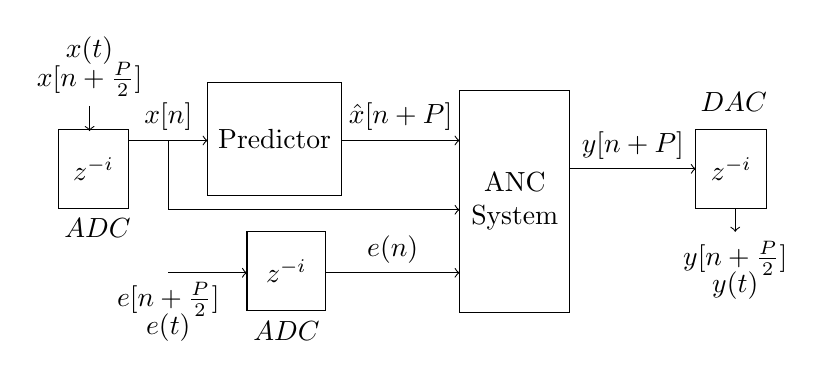
\begin{tikzpicture}
	\draw  (-3.7,1.5) rectangle node {$z^{-i}$} (-4.6,0.5);
	\draw (-4.1,0) node[above]{$ADC$} ;
	\draw (-1.7,-1.3) node[above]{$ADC$} ;
	\draw  (-2.7,2.1) rectangle  node[align=center] {\textrm{Predictor}} (-1,0.66) ;
	
	\draw  (0.5,2) rectangle node[text width=1.5cm,align=center] {\textrm{ANC System}}(1.9,-0.82);
	\draw  (3.5,1.5) rectangle node {$z^{-i}$}(4.4,0.5);
	\draw (3.98,1.6) node[above]{$DAC$} ;
	
	\draw [->](-3.7,1.36)  -- (-2.7,1.36);
	
	
	\draw [->](-1,1.36)  -- node[above]{$\hat{x}[n+P]$}  (0.5,1.36);
	\draw [->](1.9,1) -- node[above]{$y[n+P]$} (3.5,1);
	
	\draw [->](-4.2,1.8) node[above]{$x[n+\frac{P}{2}]$} -- (-4.2,1.48);
	\draw (-4.2,2.2) node[above]{$x(t)$} ;
	\draw [->](4,0.5)-- (4,0.2) node[below]{$y[n+\frac{P}{2}]$} ;
	\draw [->](-3.2,1.36) node[above]{$x[n]$} -- (-3.2,0.48) -- (0.5,0.48);
	\draw (4,-0.78) node[above]{$y(t)$} ;
	\draw  (-1.2,0.2) rectangle node {$z^{-i}$} (-2.2,-0.8);
	
	
	\draw [->](-1.2,-0.32) -- node[above]{$e(n)$} (0.5,-0.32);
	\draw [<-](-2.2,-0.32)-- (-3.2,-0.32) node[below]{$e[n+\frac{P}{2}]$} ;
	\draw (-3.2,-1.32) node[above]{$e(t)$} ;
	\end{tikzpicture}}